\section{Introduccion}

En este trabajo, se implementó un clasificador basado en una Red Convolucional Profunda para la de detección de un potencial evocado por un estímulo (Event-Related Potential, ERP). Para ello, se utilizó un dataset obtenido durante un experimento llevado a acabo en una exposición con un headset de bajo costo, lo cual permite experimentar esta técnica en un ambiente no tan controlado y más ruidoso.

\subsection{P300}

Los potenciales relacionados con eventos (Event-related potential, o ERP) son la medida de las respuestas cerebrales a eventos cognitivos, sensoriales o motores específicos. Uno de los principales enfoques relacionados con las interfases cerebro-computadora (BCI) se basa en los ERP.

Un tipo de onda bien estudiada es el P300. El potencial evocado P300 corresponde a la presencia de un pico de voltaje, del orden los uV, con una latencia cercana a los 300 ms, como se puede apreciar en la figura \ref{fig:P300Wave}. Este potencial se presente ante un estímulo visual, auditivo o sensorial ``infrecuente'', es decir, que ocurre con menor probabilidad que otros estímulos más frecuentes, a los cuáles llamaremos distractores \cite{Amiri2013ARO}.

\begin{figure}[t]
    \centering
    \begin{subfigure}{.45\textwidth}
        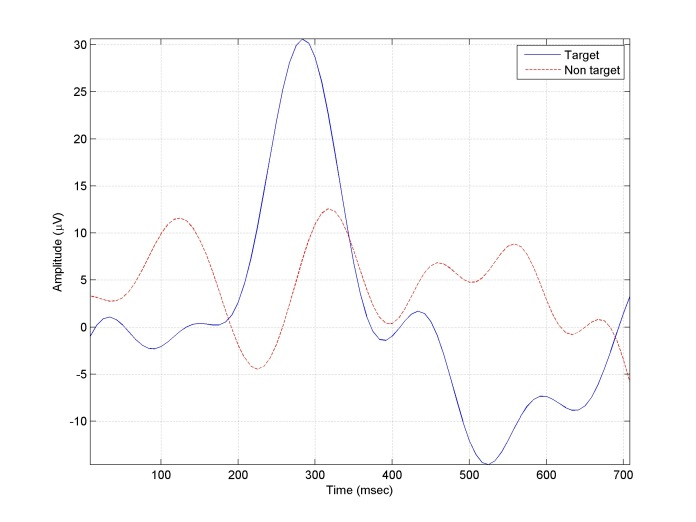
\includegraphics[width=\textwidth]{P300Wave.jpg}
        \subcaption{ Patrón temporal del componente P300..}
        \label{fig:P300Wave}
    \end{subfigure}
    
    \begin{subfigure}{.45\textwidth}
        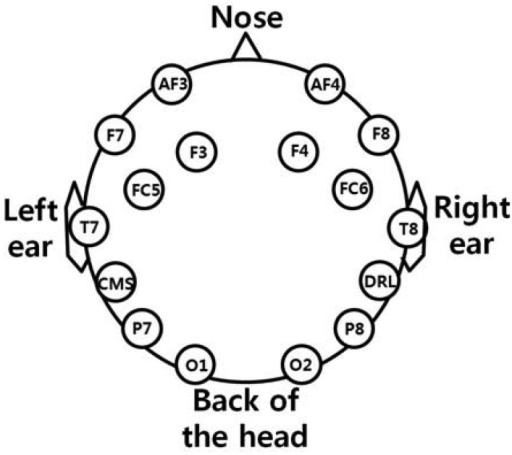
\includegraphics[width=\textwidth]{emotiv}
        \subcaption{ Loocalización de los electrodos usados para la detección de los P300.}
        \label{fig:ElectrodeMap}
    \end{subfigure}
    
\end{figure}


\subsection{P300 Speller}

 
\begin{figure}[t]
    \centering
    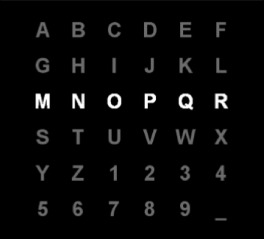
\includegraphics{Matrix6x6.jpg}
    \caption{Configuración típica de un P300 BCI con relimentación visual.}
    \label{fig:Matrix6x6}
\end{figure}

El potencial evocado P300 ha demostrado ser una señal confiable para controlar un BCI. En \cite{farwell1988talking} se describe el P300 Speller, un método de deletreo mediante BCI. Consiste en una matriz de caracteres de $6 \times 6$ como se muestra en la figura \ref{fig:Matrix6x6}. Esta matriz se presenta en la pantalla de la computadora. El usuario centra su atención en un carácter para seleccionarlo, mientras de manera aleatoria se van iluminando las 6 filas y 6 columnas. La fila o columna parpadeante correspondiente al caracter seleccionado evoca la respuesta P300. Las filas y columnas distractoras no contribuyen a generar P300. Como observamos, la frecuencia de aparición de este potencial evocado es de 1/6, ya que sólo una de las filas y una de las columnas es la objetivo mientras las demás son distractoras.

Mediante un algoritmo de clasificación, podemos predecir la probabilidad de ocurrencia de este potencial en el intervalo medido. En base a repetidos intentos (iluminando varias veces cada fila y cada columna) se puede obtener con relativa precisión el caracter en cuestión